\newpage

\anonchapter{Лабораторная работа №5}
\setcounter{chapter}{5}

\begin{center}
Исследование магнетосопротивления полупроводников\\
(4 часа)
\end{center}

\section{Цель работы}
Измерение изменения сопротивления полупроводников в магнитном поле, определение дрейфовой подвижности носителей заряда.

\section{Теоретическая часть}

\subsection{Увеличение электросопротивления полупроводника в магнитном поле}

Эффект магнетосопротивления заключается в изменении электросопротивления обазца при наложении магнитного поля. Причиной возникновения этого эфекта является искривление траектории движения носителей заряда в скрещенных магнитном и электрическом полях.

\begin{figure}[h!]\centering
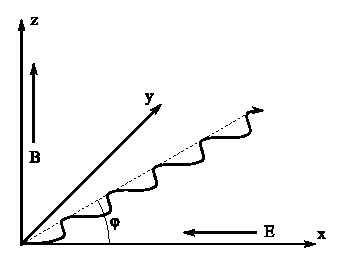
\includegraphics[height=6cm]{pic5_cycloid.eps}
\caption{Траектория электрона в скрещенных электрическом и магнитном полях внутри неограниченного полупроводника}
\label{pic5_cycloid}
\end{figure}

На движущийся заряд в магнитном поле действует сила Лоренца, которая направлена перпендикулярно дрейфовой скорости электронов $\overrightarrow{V}_{d}$ и вектору магнитной индукции $\overrightarrow{B}$. В полупроводнике заряд не может двигаться сколь угодно долго вдоль идеальной траектории, так как испытывает периодические столкновения с дефектами кристаллической решётки. При столкновении теряется энергия и, следовательно, скорость. Таким образом, носители заряда в кристалле двигаются по отрезкам циклоиды (см. рисунок \ref{pic5_cycloid}), при этом среднее направление их движения составляет с направлением поля $\overrightarrow{E}$ некоторый угол $\phi$, называемый углом Холла. Величина угла Холла определяется соотношением между дрейфовой подвижностью носителей $\mu_{d} $ и индукцией магнитного поля:

\begin{equation}
\tg \phi = \mu_{d} B
\end{equation}

Из-за того, что частица движется не по прямой, за время свободного пробега она проходит вдоль поля расстояние меньшее, чем длина свободного пробега $l_{0}$:

\begin{equation}
l_{\text{х}} = l_{0} \cos \phi
\end{equation}

В слабых магнитных полях при малом значении угла Холла

\begin{equation}
l_{\text{х}} = l_{0} \left( 1-\frac{\phi^2}{2} \right) = l_{0} \left( 1-\frac{\mu_{d}^2 B^2}{2} \right)
\end{equation}

Уменьшение пути $l_{\text{х}}$ эквивалентно уменьшению проводимости проводника:

\begin{equation}
\frac{\Delta \rho}{\rho_{0}} = \frac{\rho_{B} - \rho_{0}}{\rho_{0}} = \frac{\sigma_{0} - \sigma_{B}}{\sigma_{B}} = \frac{\l_{0} - \l_{\text{х}}}{\l_{\text{х}}} \approx \frac{\mu_{d}^2 B^2}{2}
\end{equation}

Изменение электросопротивления полупроводника пропорционально квадрату индукции магнитного поля, при этом коэффициент пропорциональности определяется величиной дрейфовой подвижности.

\subsection{Величина магнетосопротивления в ограниченном полупроводнике}

\begin{figure}[h!]\centering
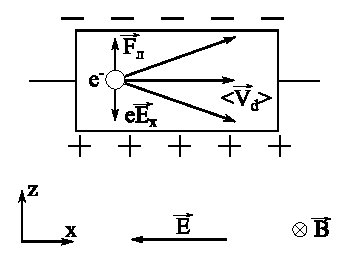
\includegraphics[height=6cm]{pic5_strip.eps}
\caption{Направления движения электронов в ограниченном образце в скрещенных электрическом и магнитном полях}
\label{pic5_strip}
\end{figure}

Рассмотрим полупроводник в виде длинного однородного стержня (рис. \ref{pic5_strip}). Под действием электрического поля $\overrightarrow{E}$ электроны движутся вдоль оси $x$. Со стороны магнитного поля $\overrightarrow{B} \perp \overrightarrow{E}$ на электроны действует сила Лоренца, направленная вдоль оси $z$. Двигаясь под действием силы Лоренца электроны скапливаются на одной из граней, заряжая её отрицательно. На противоположной грани образцется положительный заряд нескомпенсированных ионов примеси. В результате возникает поперечная ЭДС Холла, препятствующая дальнейшему разделению зарядов. Накопление зарядов будет продолжаться до тех пор, пока поле Холла не скомпенсирует отклоняющее действие магнитного поля:

\begin{equation}
e \overrightarrow{E} = -e \left[ \overrightarrow{V}_{d} \times \overrightarrow{B} \right]
\end{equation}

Если бы все электроны в кристалле имели одинаковые скорости, то они двигались бы прямолинейно вдоль оси Ox, так как кулоновская сила создаваемая полем Холла уравновешивается силой Лоренца. Однако в полупроводнике всегда имеет место некоторое распределение электронов по скоростям, обусловленное вероятностным характером рассеяния носителей. Из-за этого электроны, обладающие скоростью ниже средней будут отклоняться к одной грани образца под действием нескомпенсированного поля Холла, а обладающие более высокой скоростью - к другой, под действием нескомпенсированной силы Лоренца. При этом поток электронов в направлении приложенного поля уменьшается, что приводит к уменьшению электропроводности. За счёт того, что продольная скорость уменьшается только для электронов со скоростями, далёкими от средней, увеличение электросопротивления будет менее заментым, нежели в неограниченном образце. В вырожденных полупроводниках и металлах в проводимости участвуют прежде всего электроны, находящиеся вблизи уровня Ферми и обладающие поэтому практически одинаковыми скоростями, поэтому эффект Холла в них будет заметен гораздо меньше, чем в невырожденных полупроводниках.

Более строгий вывод эффекта магнетосопротивления может быть проведён на основе решения кинетического уравнения Больцмана. Решением являются выражения для электропроводности в присутствии магнитного поля

\begin{equation}
\sigma_{B} = e n \left< \frac{\mu}{1 + \mu^2 B^2} \right>
\end{equation}

В области слабых магнитных полей ($\mu B \ll 1$) 

\begin{equation}
\frac{\Delta \rho}{\rho_{0}} = \frac{<\mu^3>}{<\mu>} B^2 = \frac{<\mu^3>}{<\mu>^3}\mu^{2}_{d} B^2 = \frac{<\tau^3>}{<\tau>^3}\mu^{2}_{d} B^2 = C \mu^{2}_{d} B^2
\end{equation}

Величина $C$ характеризует разброс носителей по скоростям и определяется доминирующим механизмом рассеяния.

В сильном магнитном поле ($\mu B \gg 1$) 

\begin{equation}
\frac{\Delta \rho}{\rho_{0}} = \frac{<\mu>}{<\mu^{-1}>} B^2 = \frac{1}{<\mu><\mu^{-1}>} \mu_{d}^2 B^2 = \frac{1}{<\tau><\tau^{-1}>} \mu_{d}^2 B^2
\end{equation}

для ограниченного полупроводника с одним типом носителей, имеющего форму бесконечно длинного стержня, в области слабых магнитных полей ($\mu B \ll 1$) можно считать, что

\begin{equation}
\frac{\Delta \rho}{\rho_{0}} = [C - A^2] \mu^{2}_{d} B^2
\end{equation}
где $C = \frac{\left< \tau^3 \right>}{\left< \tau \right>^3}$, $A = \frac{\left< \tau^2 \right>}{\left< \tau \right>^2}$ - холл-фактор.

\subsection{Диск Корбино}
Удобной моделью неограниченного образца является диск Корбино - образец, выполненный в форме диска с отверстием в центре (рис. \ref{pic5_korbino}). Токовые контакты в таком образце расположены в центральном отверстии и по периферии диска, а магнитное поле направлено перпендикулярно плоскости диска. Линии тока наравлены от цента к краям по радиусу. Под действием магнитного поля линии тока в образце искривляются, но поперечное к электрическому поле Холла не возникает, так как не происходит разделения зарядов в образце.